\documentclass[a4paper, 12pt]{article}

% packages
\usepackage{amssymb}
\usepackage[fleqn]{mathtools}
\usepackage{tikz}
\usepackage{enumerate}
\usepackage{bussproofs}
\usepackage{xcolor}
\usepackage[margin=1.3cm]{geometry}
\usepackage{logicproof}
\usepackage{diagbox}
\usepackage{listings}
\usepackage{graphicx}
\usepackage{lstautogobble}
\usepackage{hyperref}
\usepackage{multirow}
\usepackage{tipa}
\usepackage{pgfplots}
\usepackage{adjustbox}
\usepackage{dsfont}

% tikz libraries
\usetikzlibrary{
    decorations.pathreplacing,
    arrows,
    shapes,
    shapes.gates.logic.US,
    circuits.logic.US,
    calc,
    automata,
    positioning,
    intersections
}

\pgfplotsset{compat=1.16}

\pgfmathdeclarefunction{gauss}{2}{%
  \pgfmathparse{1/(#2*sqrt(2*pi))*exp(-((x-#1)^2)/(2*#2^2))}%
}

\allowdisplaybreaks % allow environments to break
\setlength\parindent{0pt} % no indent

% shorthand for verbatim
% this clashes with logicproof, so maybe fix this at some point?
\catcode`~=\active
\def~#1~{\texttt{#1}}

% code listing
\lstdefinestyle{main}{
    numberstyle=\tiny,
    breaklines=true,
    showspaces=false,
    showstringspaces=false,
    tabsize=2,
    numbers=left,
    basicstyle=\ttfamily,
    columns=fixed,
    fontadjust=true,
    basewidth=0.5em,
    autogobble,
    xleftmargin=3.0ex,
    mathescape=true
}
\newcommand{\dollar}{\mbox{\textdollar}} %
\lstset{style=main}

% augmented matrix
\makeatletter
\renewcommand*\env@matrix[1][*\c@MaxMatrixCols c]{%
\hskip -\arraycolsep
\let\@ifnextchar\new@ifnextchar
\array{#1}}
\makeatother

% ceiling / floor
\DeclarePairedDelimiter{\ceil}{\lceil}{\rceil}
\DeclarePairedDelimiter{\floor}{\lfloor}{\rfloor}

% custom commands
\newcommand{\indefint}[2]{\int #1 \, \mathrm{d}#2}
\newcommand{\defint}[4]{\int_{#1}^{#2} #3 \, \mathrm{d}#4}
\newcommand{\pdif}[2]{\frac{\partial #1}{\partial #2}}
\newcommand{\dif}[2]{\frac{\mathrm{d}#1}{\mathrm{d}#2}}
\newcommand{\limit}[2]{\raisebox{0.5ex}{\scalebox{0.8}{$\displaystyle{\lim_{#1 \to #2}}$}}}
\newcommand{\limitsup}[2]{\raisebox{0.5ex}{\scalebox{0.8}{$\displaystyle{\limsup_{#1 \to #2}}$}}}
\newcommand{\summation}[2]{\sum\limits_{#1}^{#2}}
\newcommand{\product}[2]{\prod\limits_{#1}^{#2}}
\newcommand{\intbracket}[3]{\left[#3\right]_{#1}^{#2}}
\newcommand{\laplace}{\mathcal{L}}
\newcommand{\fourier}{\mathcal{F}}
\newcommand{\mat}[1]{\boldsymbol{#1}}
\renewcommand{\vec}[1]{\boldsymbol{#1}}
\newcommand{\rowt}[1]{\begin{bmatrix}
    #1
\end{bmatrix}^\top}
\DeclareMathOperator*{\argmax}{argmax}
\DeclareMathOperator*{\argmin}{argmin}

\newcommand{\lto}[0]{\leadsto\ }

\newcommand{\ulsmash}[1]{\underline{\smash{#1}}}

\newcommand{\powerset}[0]{\wp}
\renewcommand{\emptyset}[0]{\varnothing}

\makeatletter
\newsavebox{\@brx}
\newcommand{\llangle}[1][]{\savebox{\@brx}{\(\m@th{#1\langle}\)}%
  \mathopen{\copy\@brx\kern-0.5\wd\@brx\usebox{\@brx}}}
\newcommand{\rrangle}[1][]{\savebox{\@brx}{\(\m@th{#1\rangle}\)}%
  \mathclose{\copy\@brx\kern-0.5\wd\@brx\usebox{\@brx}}}
\makeatother
\newcommand{\lla}{\llangle}
\newcommand{\rra}{\rrangle}
\newcommand{\la}{\langle}
\newcommand{\ra}{\rangle}
\newcommand{\crnr}[1]{\text{\textopencorner} #1 \text{\textcorner}}
\newcommand{\bnfsep}[0]{\ |\ }
\newcommand{\concsep}[0]{\ ||\ }

\newcommand{\axiom}[1]{\AxiomC{#1}}
\newcommand{\unary}[1]{\UnaryInfC{#1}}
\newcommand{\binary}[1]{\BinaryInfC{#1}}
\newcommand{\trinary}[1]{\TrinaryInfC{#1}}
\newcommand{\quaternary}[1]{\QuaternaryInfC{#1}}
\newcommand{\quinary}[1]{\QuinaryInfC{#1}}
\newcommand{\dproof}[0]{\DisplayProof}
\newcommand{\llabel}[1]{\LeftLabel{\scriptsize #1}}
\newcommand{\rlabel}[1]{\RightLabel{\scriptsize #1}}

\newcommand{\ttbs}{\char`\\}
\newcommand{\lrbt}[0]{\ \bullet\ }

% colours
\newcommand{\violet}[1]{\textcolor{violet}{#1}}
\newcommand{\blue}[1]{\textcolor{blue}{#1}}
\newcommand{\red}[1]{\textcolor{red}{#1}}
\newcommand{\teal}[1]{\textcolor{teal}{#1}}

% reasoning proofs
\usepackage{ltablex}
\usepackage{environ}
\keepXColumns
\NewEnviron{reasoning}{
    \begin{tabularx}{\textwidth}{rlX}
        \BODY
    \end{tabularx}
}
\newcommand{\proofline}[3]{$(#1)$ & $#2$ & \hfill #3 \smallskip \\}
\newcommand{\proofarbitrary}[1]{& take arbitrary $#1$ \smallskip \\}
\newcommand{\prooftext}[1]{\multicolumn{3}{l}{#1} \smallskip \\}
\newcommand{\proofmath}[3]{$#1$ & = $#2$ & \hfill #3 \smallskip \\}
\newcommand{\prooftherefore}[1]{& $\therefore #1$ \smallskip \\}
\newcommand{\proofbc}[0]{\prooftext{\textbf{Base Case}}}
\newcommand{\proofis}[0]{\prooftext{\textbf{Inductive Step}}}

% ER diagrams
\newcommand{\nattribute}[4]{
    \node[draw, state, inner sep=0cm, minimum size=0.2cm, label=#3:{#4}] (#1) at (#2) {};
}
\newcommand{\mattribute}[4]{
    \node[draw, state, accepting, inner sep=0cm, minimum size=0.2cm, label=#3:{#4}] (#1) at (#2) {};
}
\newcommand{\dattribute}[4]{
    \node[draw, state, dashed, inner sep=0cm, minimum size=0.2cm, label=#3:{#4}] (#1) at (#2) {};
}
\newcommand{\entity}[3]{
    \node[] (#1-c) at (#2) {#3};
    \node[inner sep=0cm] (#1-l) at ($(#1-c) + (-1, 0)$) {};
    \node[inner sep=0cm] (#1-r) at ($(#1-c) + (1, 0)$) {};
    \node[inner sep=0cm] (#1-u) at ($(#1-c) + (0, 0.5)$) {};
    \node[inner sep=0cm] (#1-d) at ($(#1-c) + (0, -0.5)$) {};
    \draw
    ($(#1-c) + (-1, 0.5)$) -- ($(#1-c) + (1, 0.5)$) -- ($(#1-c) + (1, -0.5)$) -- ($(#1-c) + (-1, -0.5)$) -- cycle;
}
\newcommand{\relationship}[3]{
    \node[] (#1-c) at (#2) {#3};
    \node[inner sep=0cm] (#1-l) at ($(#1-c) + (-1, 0)$) {};
    \node[inner sep=0cm] (#1-r) at ($(#1-c) + (1, 0)$) {};
    \node[inner sep=0cm] (#1-u) at ($(#1-c) + (0, 1)$) {};
    \node[inner sep=0cm] (#1-d) at ($(#1-c) + (0, -1)$) {};
    \draw
    ($(#1-c) + (-1, 0)$) -- ($(#1-c) + (0, 1)$) -- ($(#1-c) + (1, 0)$) -- ($(#1-c) + (0, -1)$) -- cycle;
}

% AVL Trees
\newcommand{\avltri}[4]{
    \draw ($(#1)$) -- ($(#1) + #4*(0.5, -1)$) -- ($(#1) + #4*(-0.5, -1)$) -- cycle;
    \node at ($(#1) + #4*(0, -1) + (0, 0.5)$) {#3};
    \node at ($(#1) + #4*(0, -1) + (0, -0.5)$) {#2};
}

% RB Trees
\tikzset{rbtr/.style={inner sep=2pt, circle, draw=black, fill=red}}
\tikzset{rbtb/.style={inner sep=2pt, circle, draw=black, fill=black}}

% Samples
\tikzset{spos/.style={inner sep=2pt, circle, draw=black, fill=blue!20}}
\tikzset{sneg/.style={inner sep=2pt, circle, draw=black, fill=red!20}}

% Joins
\newcommand\ljoin{\stackrel{\mathclap{\normalfont\mbox{\tiny L}}}{\bowtie}}
\newcommand\rjoin{\stackrel{\mathclap{\normalfont\mbox{\tiny R}}}{\bowtie}}
\newcommand\ojoin{\stackrel{\mathclap{\normalfont\mbox{\tiny O}}}{\bowtie}}

\setcounter{MaxMatrixCols}{100}

% actual document
\begin{document}
    {\sc Computing $4^\text{th}$ Year Notes} \hfill ~https://github.com/lin-e/imperial-revision~
    \rule{\textwidth}{0.1pt}
    \section*{Reinforcement Learning \hfill (70028)}
        \subsection*{Markov Processes (Let's Go Markov)}
            In reinforcement learning, we need a real, tangible method for managing complexity.
            It's important to distinguish between \textbf{Markov Processes} and \textbf{Markov Decision Processes}.
            \medskip

            A Markov process is a tuple $(\mathcal{S}, \mathcal{P})$, where $\mathcal{S}$ is a set of states, and $\mathcal{P}_{ss^\prime}$ is a matrix giving us the probability of transitioning from one state to another; note that the probabilities are based only on the current state (one at time $t$), and not looking beyond that - short memory is important;
            $$\mathcal{P}_{ss^\prime} = P [S_{t + 1} = s^\prime\ \vline\ S_t = s]$$
            A Markov process generates a chain of states governed by probabilistic transitions.
            \medskip

            A state $s_t$ is Markov iff $P[s_{t + 1}\ \vline\ s_t] = P[s_{t + 1}\ \vline\ s_1, \dots, s_t]$; the conditional probability of transitioning to a particular state depends only on the particular state (previous states don't really matter).
            The equation states that the probabilities are equal, whether it be the current state, or all states preceding - the future is independent of the past given the present.
            Another way this can be thought of is that the present state, $s_t$, captures all information in the history of the agent's events, any data of the history is no longer needed once the state is known, or the current state is a sufficient statistic of the future.
            \medskip

            An example is as follows, note that the black states are transient states (where it can lead to another state) and the \violet{violet} states are terminal states.
            The following is Markovian as the probabilities don't change based on the history (how we got to a state).
            \begin{center}
                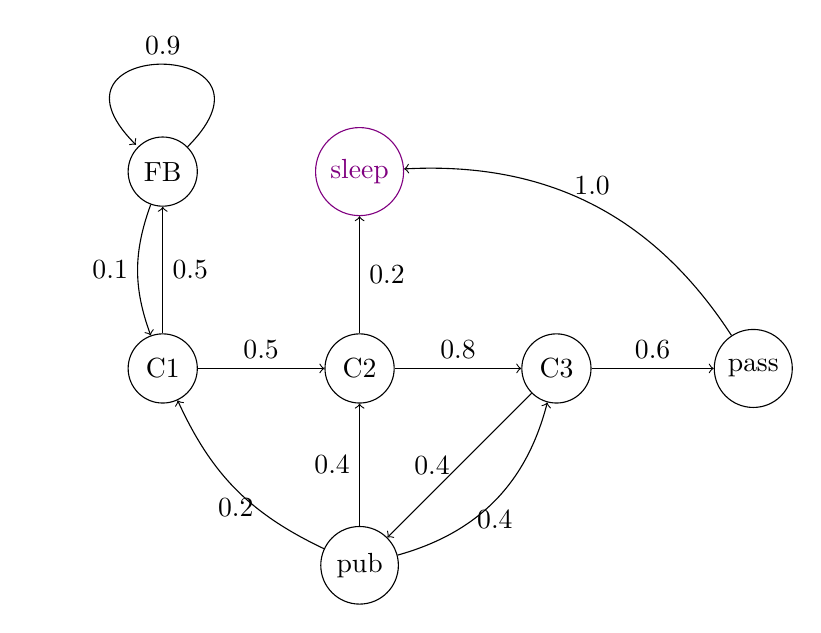
\begin{tikzpicture}[x=2.5cm, y=2.5cm]
                    \node[state] (fb) at (0, 0) {FB};
                    \node[state] (c1) at (0, -1) {C1};
                    \node[state] (c2) at (1, -1) {C2};
                    \node[state] (c3) at (2, -1) {C3};
                    \node[state] (p) at (3, -1) {pass};
                    \node[state] (pub) at (1, -2) {pub};
                    \node[state, violet] (sleep) at (1, 0) {sleep};

                    \draw
                    (c1) edge[->, right] node{$0.5$} (fb)
                    (fb) edge[->, bend right=20, left] node{$0.1$} (c1)
                    (fb) edge[loop, ->, above] node{$0.9$} (fb)
                    (c1) edge[->, above] node{$0.5$} (c2)
                    (c2) edge[->, above] node{$0.8$} (c3)
                    (c3) edge[->, above] node{$0.6$} (p)
                    (p) edge[->, bend right=30, above] node{$1.0$} (sleep)
                    (c2) edge[->, right] node{$0.2$} (sleep)
                    (pub) edge[->, bend left=20, below] node{$0.2$} (c1)
                    (pub) edge[->, left] node{$0.4$} (c2)
                    (pub) edge[->, bend right=30, below] node{$0.4$} (c3)
                    (c3) edge[->, left] node{$0.4$} (pub);
                \end{tikzpicture}
            \end{center}
            The entries must be probabilities (hence between 0 and 1).
            The matrix defines transition probabilities from all states $s$ to all successor states $s^\prime$.
            Since all probabilities have to be accounted for (all rows of the matrix sum to 1) - after leaving $s$, we need to end up somewhere, which could also mean returning to $s$;
            $$\summation{s^\prime}{} \mathcal{P}_{ss^\prime} = 1$$
            In the example above, the probability of going to sleep after C2 (class 2) in the morning could be different depending on the time of day (i.e. constantly changing).
            If $P[s_{t + 1}\ \vline\ s_t]$ doesn't depend on $t$, but rather just the origin and destination states, then the Markov chain is stationary or homogenous.
            \subsubsection*{Markov Reward Process}
                A Markov Reward Process is a Markov chain which emits rewards (the reward hypothesis states that all of what we think of as goals and purposes can be thought of as the maximisation of the expected value of the cumulative sum of a scalar signal known as reward); hence a tuple $(\mathcal{S}, \mathcal{P}, \mathcal{R}, \gamma)$.
                This has the following components;
                \begin{itemize}
                    \itemsep0em
                    \item $\mathcal{S}$ \hfill a set of states
                    \item $\mathcal{P}_{ss^\prime}$ \hfill a state transition probability matrix
                    \item $\mathcal{R}_s = \mathbb{E}[r_{t + 1}\ \vline\ S_t = s]$
                        \subitem an expected immediate reward, collected upon departing state $s$ (collection occurs at time $t + 1$, we are at state $s$ at time $t$)
                    \item $\gamma \in [0, 1]$ \hfill discount factor
                \end{itemize}
                We can define the return $R_t$ as the total discounted reward from time-step $t$ (note that we use $t + 1$ as the first element, since it's collected at $t + 1$);
                $$R_t = r_{t + 1} + \gamma r_{t + 2} + \dots = \summation{k = 0}{\infty} \gamma^k r_{t + k + 1}$$
                The factor $\gamma$ is how we discount the present value of future rewards; the value of receiving a reward $r$ after $k + 1$ time steps is $\gamma^k r$, valuing immediate reward higher than a delayed reward - hence $\gamma$ closer to 0 leads to short-sighted evaluation, whereas $\gamma$ closer to 1 leads to far-sighted evaluation (taking future rewards more strongly).

                \medskip
                We can add a reward to the previous example as follows (in \red{red});
                \begin{center}
                    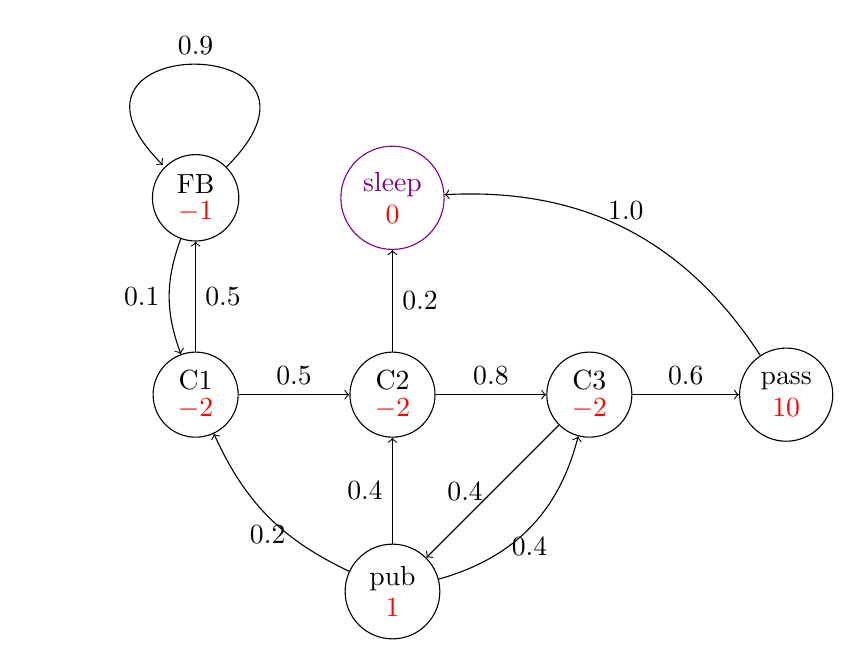
\begin{tikzpicture}[x=2.5cm, y=2.5cm]
                        \node[state] (fb) at (0, 0) {\shortstack{FB\\\red{$-1$}}};
                        \node[state] (c1) at (0, -1) {\shortstack{C1\\\red{$-2$}}};
                        \node[state] (c2) at (1, -1) {\shortstack{C2\\\red{$-2$}}};
                        \node[state] (c3) at (2, -1) {\shortstack{C3\\\red{$-2$}}};
                        \node[state] (p) at (3, -1) {\shortstack{pass\\\red{$10$}}};
                        \node[state] (pub) at (1, -2) {\shortstack{pub\\\red{$1$}}};
                        \node[state, violet] (sleep) at (1, 0) {\shortstack{sleep\\\red{$0$}}};

                        \draw
                        (c1) edge[->, right] node{$0.5$} (fb)
                        (fb) edge[->, bend right=20, left] node{$0.1$} (c1)
                        (fb) edge[loop, ->, above] node{$0.9$} (fb)
                        (c1) edge[->, above] node{$0.5$} (c2)
                        (c2) edge[->, above] node{$0.8$} (c3)
                        (c3) edge[->, above] node{$0.6$} (p)
                        (p) edge[->, bend right=30, above] node{$1.0$} (sleep)
                        (c2) edge[->, right] node{$0.2$} (sleep)
                        (pub) edge[->, bend left=20, below] node{$0.2$} (c1)
                        (pub) edge[->, left] node{$0.4$} (c2)
                        (pub) edge[->, bend right=30, below] node{$0.4$} (c3)
                        (c3) edge[->, left] node{$0.4$} (pub);
                    \end{tikzpicture}
                \end{center}
                For example, consider a certain run, where the starting state $S_1 = \text{C1}$ and $\gamma = \frac{1}{2}$, $T$ is the time to reach the terminal state;
                $$R_1 = r_2 + \gamma r_3 + \dots + \gamma^{T - 2}r_T$$
                Consider the run where the student attends all classes in order and passes; hence C1, C2, C3, pass, sleep;
                $$R_1 = -2 + \frac{1}{2} \cdot -2 + \frac{1}{2}^2 \cdot -2 + \frac{1}{2}^3 \cdot 10$$
                Most MRPs are discounted with $\gamma < 1$, as it's mathematically convenient by avoiding infinite returns in cyclic / infinite processes (by causing convergence).
                It also aids in expressing uncertainty in future rewards.
                A more tangible example is a financial reward, where immediate rewards can be put into a bank and earn interest, similarly, animal decision making shows preference for immediate rewards rather than future rewards.
                \medskip

                We can define the state value function $v(s)$ of a MRP as the expected return $R$ starting from state $s$ at time $t$, thinking of the state as a function parameter;
                $$v(s) = \mathbb{E}[R_t\ \vline\ S_t = s]$$
                The lecture then goes over an example using golf, which is actually quite intuitive.
                \medskip

                The Bellman Equation for MRPs is as follows.
                We can express it in a recurrence relation, as the \violet{immediate reward} and the \teal{discounted return of the successor state}.
                \begin{align*}
                    v(s) & = \mathbb{E}[R_t\ \vline\ S_t = s] \\
                    & = \mathbb{E}[r_{t + 1} + \gamma r_{t + 2} + \gamma^2 r_{t + 3} + \dots\ \vline\ S_t = s] \\
                    & = \mathbb{E}[r_{t + 1} + \gamma(r_{t + 2} + \gamma r_{t + 3} + \dots)\ \vline\ S_t = s] \\
                    & = \mathbb{E}[r_{t + 1} + \gamma R_{t + 1}\ \vline\ S_t = s] \\
                    & = \mathbb{E}[\violet{r_{t + 1}} + \teal{\gamma v(S_{t + 1}})\ \vline\ S_t = s]
                \end{align*}
                The equation can also be written as the sum notation (the previous one was the expectation notation, this has the expectation written out) - there are a total of $n$ of these equations, as there's one for each state;
                $$v(s) = \mathcal{R}_s + \gamma \summation{s^\prime \in S}{} \mathcal{P}_{ss^\prime}v(s^\prime)$$
                As such, this can be written in vector notation as follows, with $\vec{v}$ being $n$-dimensional;
                $$\vec{v} = \mathcal{R} + \gamma \mathcal{P} \vec{v}$$
                This can be directly solved as follows, as it's linear and self-consistent;
                \begin{align*}
                    \vec{v} & = \mathcal{R} + \gamma \mathcal{P} \vec{v} \\
                    (\mathds{1} - \gamma \mathcal{P}) \vec{v} & = \mathcal{R} \\
                    \vec{v} & = (\mathds{1} - \gamma \mathcal{P})^{-1} \mathcal{R}
                \end{align*}
                Since matrix inversion is computationally expensive, being in the order of $n^3$ for $n$ states, a direct solution is only feasibly for small MRPs.
                Iterative methods for solving large MRPs include (and all three will be covered);
                \begin{itemize}
                    \itemsep0em
                    \item dynamic programming
                    \item Monte-Carlo evaluation
                    \item Temporal-Difference learning
                \end{itemize}
            \subsubsection*{Policies}
                A policy $\pi$ is a function of the state, formalising the actions to take at a given state.
                A rigid, deterministic policy can be disadvantageous (e.g. rock, paper, scissors) - exposing the agent to being systematically exploited.
                A policy can be formally described as the conditional probability distribution to execute an action $a \in \mathcal{A}$ given that one is in state $s \in \mathcal{S}$ at time $t$;
                $$\pi_t(a, s) = P[A_t = a\ \vline\ S_t = s]$$
                The general form of the policy is probability, or stochastic, hence $\pi$ is a probability.
                However, if the policy is deterministic (only a single $a$ is possible for state $s$), then $\pi(a, s) = 1$, $\pi(a^\prime, s) = 0,\ \forall a \neq a^\prime$.
                \medskip

                Consider the following example, where there are two actions, $a_1, a_2$ where we either play the lottery (costing 1), or save (not costing anything).
                The two states, $s_1$ and $s_2$ correspond to winning or losing the lottery.
                $$a^* = \argmax_{a_i} \summation{j = 1}{2} \mathcal{R}_{s_j}^{a_j}P[s_j\ |\ a_i]$$
 \end{document}